\documentclass[]{scrreprt}
\usepackage{amsmath,amsfonts,graphicx}
\usepackage{multirow}
\usepackage{pslatex}
\usepackage{tabularx}
\usepackage{comment}
\usepackage{xspace}
\usepackage{array}

\usepackage{hyperref}

\usepackage{caption}
\DeclareCaptionFont{white}{\color{white}}
\DeclareCaptionFormat{listing}{\colorbox{gray}{\parbox{\textwidth}{#1#2#3}}}

\graphicspath{
{figures/}
}

\newcommand{\uo}{\mbox{UO\textsubscript{2}}\xspace}

\setcounter{secnumdepth}{3}


\begin{document}


\title{Richards Theory Manual}
\author{Andy Wilkins \\
CSIRO}
\maketitle

\tableofcontents

%%%
\chapter{Introduction}
%%%

The Richards' equation\footnote{Contrary to the urban legend,
  ``Richards'' is unrelated to Richard Martineau:
  see~\cite{richards1931}.} describes slow fluid flow through a porous
medium.  This document describes the theoretical and numerical
foundations of the MOOSE implementation.
\begin{itemize}
\item Chapter~\ref{chap.govern.eqn} describes the governing equation
  and associated nonlinear functions.
\item Chapter~\ref{sources.sinks.chap} describes the sources and sinks
  that I have implemented.
\item Chapter~\ref{chap.upwinding} describes upwinding
\item Chapter~\ref{discret.chap} describes the discretisation of the time derivative.
\item Chapter~\ref{chap.multi} describes the multi-phase Richards'
  equations that I have implemented.  For notational simplicity, the
  rest of this document focusses on the single-phase case, but this
  chapter shows the multi-phase version is a straightforward
  generalisation.
\item Chapter~\ref{tol.chap} briefly discusses tolerancs and
  convergence criteria.
\end{itemize}
There are two other accompanying documents: (1) A description of the
unit tests and benchmark verifications; (2) Examples of input syntax
that users can utilise when building models.

%%%
\chapter{Governing equations for the single-phase situation}
\label{chap.govern.eqn}
%%%
The Richards' equation~\cite{richards1931} describes the movement of
fluid through the connected pore space of a porous medium.  For a
single phase, the equation is
\begin{equation}
\phi \frac{\partial}{\partial t} \left( \rho S \right) = \nabla_{i}
\left( \frac{\rho \kappa_{ij}\kappa_{\mathrm{rel}}}{\mu} (\nabla_{j}P - \rho g_{j}) \right)
+ F \ ,
\label{richards.eqn}
\end{equation}
where the independent variable is $P$, the fluid pressure.  The
multi-phase version is very similar and is described in
Chapter~\ref{chap.multi}.  On the
right-hand side, the index summation convection has been used, so $i$
and $j$ are both summed from 1 to 3 in three dimensions (or 1 to 2 in
two dimensions).  The following notation has been used.
\begin{itemize}
\item $\phi$ is the porosity of the medium (dimensionless).  It is a
  material property (independent of the fluid pressure).  The porous
  medium is assumed to be made up of solid material with a porespace
  through which the fluid can flow, and the porosity is
  $V_{\mathrm{porespace}}/V_{\mathrm{medium}}$.  The porosity is assumed
  time-independent, but may be spatially varying.  A typical value for
  rock is 0.1.  To be strict, $\phi$ is the {\em connected} porosity, as the
  medium may have disconnected pores which are irrelevant for the
  fluid flow, and will be ignored in the following.
\item $t$ is time.
\item ${\mathbf{x}}$ is space, and $\nabla_{i}$ is the gradient operator.
\item $\rho$ is the fluid density (measured in mass.length$^{-3}$,
  usually kg.m$^{-3}$).  $\rho$ is
  typically a function of pressure, which is discussed in more detail below.
\item $S$ is the fluid saturation (dimensionless).  It is bounded,
  $0\leq S \leq 1$, and is the fraction of pore volume that is filled
  with the fluid.  Hence $\phi\rho S$ appearing on the LHS of
  Richards' equation is the volume-density of fluid at a point.  The term ``fully
  saturated'' means $S=1$, so that the entire pore volume is filled
  with the fluid.  When $S<1$, the medium is called ``partially
  saturated''.  The porevolume of a partially saturated medium is
  filled partially with the fluid, and partially with another fluid
  which I shall call air in the following (the other fluid need not
  actually be air, but is convenient to call it so).  In the
  single-phase version, this air is free
  to move throughout the porevolume --- it may even be spontaneously
  created in a region where there was previously no air --- and the
  assumption of Richards' equation is that it has no affect on the
  dynamics of the fluid.   In the multi-phase version
  (Chapter~\ref{chap.multi}), the air is given a dynamics of its own.
  $S$ is a function of fluid pressure and is discussed in more detail below.
\item $\kappa_{ij}$ is the permeability tensor of the medium (measured
  in length$^{2}$, usually m$^{2}$).  It is a material property
  (independent of the fluid pressure).  It may be spatially varying.
  It is usually diagonal, since the axes ${\mathbf{x}}$ are chosen in
  its principal directions.  In groundwater scenarios it is often only
  transversely isotropic, so that $K_{xx}=K_{yy}\neq K_{zz}$.  Typical
  values for rocks are $K_{xx} = K_{yy} = 10^{-14}\,\mathrm{m}^{2}$
  and $K_{zz} = 10^{-15}\,\mathrm{m}^{2}$, although rocks with
  permeability up to six orders of magnitude greater or less than
  these values are common.
\item $\kappa_{\mathrm{rel}}$ is the relative permeability
  (dimensionless).  It is bounded $0\leq \kappa_{\mathrm{rel}} \leq 1$
  as is a function of fluid saturation.  It is discussed in more
  detail below.
\item $\mu$ is the fluid's dynamic viscosity (measured
  force.length$^{-2}$.time, usually Pa.s).  While in reality it may be
  a function of pressure, I have implemented it as constant.  A typical
  value for liquid water is $10^{-3}$\,Pa.s.
\item $P$ is the fluid porepressure (measured force.length$^{-2}$,
  usually Pa).  It is the independent variable.
\item ${\mathbf{g}}$ is the acceleration of gravity (measured
  in length.time$^{-2}$, usually m.s$^{-2}$) as a vector pointing ``downwards''.  It is constant.
  For instance
  ${\mathbf{g}} = (0,\ 0,\ -9.8)$\,m.s$^{-2}$.
\item $F$ is a source term (measured in
  mass.length$^{-3}$.time$^{-1}$, for instance kg.m$^{-3}$.s$^{-1}$).
\end{itemize}


\section{Residual saturations, effective saturation, and immobile saturation}

Although physically the fluid saturation, $S$, can never exceed its
bounds, $0\leq S\leq 1$, in practice it is sometimes found that
\begin{equation}
S_{\mathrm{res}} \leq S \leq 1 - S_{\mathrm{air}} \ .
\end{equation}
Here $S_{\mathrm{res}}$ is termed the ``residual saturation'', and
$S_{\mathrm{air}}$ is the ``residual air saturation''.

The residual saturation is attained in experiments by applying an
``infinite negative fluid pressure'' to the porous material to suck out as
much fluid as possible.  What may happen is that the fluid becomes
discontinuous so that small blobs or very thin films of fluid exist in
the material, but because they are discontinuous they do not feel
the ``infinite negative pressure''.  This gives rise to the nonzero
$S_{\mathrm{res}}$.  However, further fluid may be
extracted through other means such as heating or mechanical
stimulation.

The residual air saturation may be nonzero because as water is pumped
into an unsaturated medium, air might be trapped so the saturation
might not be able to attain $S=1$.

For $S<S_{\mathrm{res}}$ Richards' equation~(\ref{richards.eqn}) is no
longer valid as pressure can no longer be transmitted through the
fluid.  It is convenient to define the effective saturation
\begin{equation}
S_{\mathrm{eff}} = \frac{S - S_{\mathrm{res}}}{1 - S_{\mathrm{air}} -
  S_{\mathrm{res}}} \ ,
\end{equation}
which has bounds $0\leq S_{\mathrm{eff}} \leq 1$ in the domain of
applicability of Richards' equation.

It is a moot point as to whether
$S_{\mathrm{res}}=0=S_{\mathrm{air}}$, because experiments are hard to
perform.  What is of more practical use is the ``immobile
saturation'', $S_{\mathrm{imm}}$, below which the relative
permeability is zero, and that is discussed further in
Section~\ref{rel.perm.sec}.  (The physical reasons for the relative
permeability going to zero below $S_{\mathrm{imm}}$ are probably those
given above: the continuous film of fluid breaking down in the
presence of large negative porepressures.)


\section{Density}
\label{sec.density.constk}

The MOOSE implementation allows users to specify arbitrary
relationships between density and porepressure.  One common case
for liquids is that the fluid bulk modulus is constant, which means
that 
\begin{equation}
\rho = \rho_{0}e^{P/K} \ .
\end{equation}
In this expression
\begin{itemize}
\item $\rho_{0}$ is a constant reference density (measured in
  mass.length$^{-3}$).  A typical value for water is
  $10^{3}$\,kg.m$^{-3}$.
\item $P$ is the fluid porepressure.
\item $K$ is the fluid bulk modulus.  A typical value for water is
  2\,GPa.
\end{itemize}

The density of an ideal fluid (gas) has also been coded into MOOSE.

The density of a van der Waals gas has also been coded into MOOSE.

\section{Capillary suction}

Because of the different wetability of the fluid and air, there will
be capillary effects in the medium.  In an unsaturated medium, this
allows definition of the capillary pressure
\begin{equation}
P_{\mathrm{c}} = P_{\mathrm{air}} - P \ ,
\end{equation}
in terms of the air pressure and the fluid porepressure.  For the
single-phase case it is convenient to define
\begin{equation}
P_{\mathrm{air}} = 0 \ ,
\label{eqn.pair.zero}
\end{equation}
so that the porepressure is referenced to this constant air pressure.
The situation is more complicated in the multi-phase case as discussed
in Chapter~\ref{chap.multi}.

For an unsaturated wetting fluid, $P_{\mathrm{c}} > 0$, and
Laplace showed that $P_{\mathrm{c}} \propto 1/r$, where $r$ is the
radius of the capillary.  This $P_{\mathrm{c}}$ is unbounded as
$r\rightarrow 0$, but clearly there must be some cutoff where the
fluid undergoes some physical change (like boiling), as porepressures
can never actually go below a vacuum.  Alternately, it may be that for
such small scales ($r\rightarrow 0$), the concept of pressure becomes
meaningless.  This is ignored in many parts of the literature.
Indeed, as we shall see below, the relative permeability tends
strongly to zero at $P_{\mathrm{c}} \rightarrow \infty$, so it is
difficult to envisage a real-life scenario where porepressures are
less than zero (van Genuchten writes the region
$P_{\mathrm{c}} \rightarrow \infty$ is ``fairly unimportant for most
practical field problems'').

For porous materials, the capillary pressure is usually thought of as
a function of saturation.  Physically I suppose this is because of the
distribution of pore-throat sizes: many pore throats can support a
relatively small $P_{\mathrm{c}}$, while only the small pore throats
can contribute towards a large $P_{\mathrm{c}}$.  Hence, for large
$P_{\mathrm{c}}$, the fluid is only occupying a small fraction of pore
space.

Various relationships between $P_{\mathrm{c}}$ and $S_{\mathrm{eff}}$
have been proposed and used, and the MOOSE implemtnation allows users
to specify any functional relationship.  The most common is due to van
Genuchten~\cite{vangenucthen1980}:
\begin{equation}
S_{\mathrm{eff}} = \left( 1 + (\alpha P_{c})^{\frac{1}{1 - m}}
\right)^{-m} \ \ \ \mbox{for}\ \ 0<m<1 \ .
\label{vg.cap.eqn}
\end{equation}
This has a corresponding relative permeability function, detailed in
Sec~\ref{rel.perm.sec}.  Sometimes the van Genuchten functions are
defined in terms of a parameter $n=1/(1-m)> 1$.

In van Genuchten's paper, he finds good fits with experimental data
for various soils and rock when the parameter $m$ ranges between about
0.5 and 0.9 (meaning $2<n<10$, roughly), and $\alpha$ is beween
$4\times 10^{-5}$\,Pa$^{-1}$ and $2\times 10^{-4}$\,Pa$^{-1}$.
Figure~\ref{van_genuchten_pc.fig} shows the shape of the van Genuchten
suction, $P_{c}$, as a function of $S_{\mathrm{eff}}$.

Numerically there are three important features of
Eqn~(\ref{vg.cap.eqn}).
\begin{enumerate}
\item $S_{\mathrm{eff}}$ is a monotonically decreasing function of
  $P_{c}$, which is necessary for a unique solution.
\item $P_{c}\rightarrow \infty$ as $S_{\mathrm{eff}}\rightarrow 0$.  As mentioned
above, this is not justifiable physically, but numerically it is
extremely advantageous over $P_{c}\rightarrow P_{c}^{0}<\infty$, as
this latter version often causes algorithms to ``get stuck'' around
$S_{\mathrm{eff}} = 0$.  As also mentioned above, because of the low
relative permeability around $S_{\mathrm{eff}}$, physically realistic
problems rarely explore the $S_{\mathrm{eff}}\sim 0$ region.
\item $S_{\mathrm{eff}}\rightarrow 1$ and
  $\mathrm{d}S_{\mathrm{eff}}/\mathrm{d}P_{c} \rightarrow 0^{+}$ as
  $P_{c}\rightarrow 0$, for all $m$.  This ensures that there is
  continuity in the porepressure, $P$, and the derivative
  $\mathrm{d}S/\mathrm{d}P$ around full saturation (remember that by definition
  $S_{\mathrm{eff}}=1$ for $P_{c}<0$).  Also
  $\mathrm{d}^{2}S_{\mathrm{eff}}/\mathrm{d}P_{c}^{2} \rightarrow 0$
  as $P_{c}\rightarrow 0^{+}$ if $m>0.5$.  This type of term enters the
  Jacobian\footnote{It appears explicitly from the time derivative in
    Eqn~(\ref{richards.eqn}) if the derivative is written in terms of
    $\dot{P}$.  In fact, that formulation does not give good
    mass-balance characteristics so it is not used in the MOOSE implementation, but
    nevertheless it is good to have
    $\mathrm{d}^{2}S_{\mathrm{eff}}/\mathrm{d}P_{c}^{2}$ continuous.}
  in an implicit time-stepping scheme, so it is advantageous that it
  be continuous around full saturation.
\end{enumerate}
I encourage users to set $m>0.5$.

\begin{figure}[htb]
\centering
\includegraphics[width=10cm]{van_genuchten_pc.eps}
\caption{$\alpha P_{c}$ as a function of $S_{\mathrm{eff}}$ as given
  by van Genuchten's expression Eqn~(\ref{vg.cap.eqn}).  Three values
  of $m$ are shown: 0.5, 0.7 and 0.9 (the $m=0.5$ case has largest
  $P_{c}$ around $S_{\mathrm{eff}}\sim 0$).}
\label{van_genuchten_pc.fig}
\end{figure}

The Broadbridge-White capillary curve valid for small $K_{n}$ has also been coded into MOOSE~\cite{bw1988}.

The Rogers-Stallybrass-Clements capillary curve valid for zero
residual saturations and oil viscosity double that of water viscosity
has also been coded into MOOSE~\cite{rsc1983}. 

A ``shifted'' version of Eqn~(\ref{vg.cap.eqn}) has been coded for
into MOOSE for 2-phase simulations.  The effective saturation for the
``water'' phase is
\begin{equation}
S^{\mathrm{water}}_{\mathrm{eff}} = S_{s}^{-1}\left( 1 + (\alpha
  (P^{\mathrm{gas}} - P^{\mathrm{water}} + s))^{\frac{1}{1 - m}}
\right)^{-m} \ \ \ \mbox{for}\ \ 0<m<1 \ ,
\end{equation}
where $s$ is the so-called ``shift'', and $S_{s}$ is the value of
Eqn~(\ref{vg.cap.eqn}) at $P_{c}=s$ (so $S_{s}^{-1}$ scales the result so
that $0\leq S_{\mathrm{eff}}\leq 1$).  The ``gas'' saturation is just
$S^{\mathrm{gas}}_{\mathrm{eff}}=1-S^{\mathrm{water}}_{\mathrm{eff}}$.
Here it assumed that $P_{c} = P^{\mathrm{gas}}-P^{\mathrm{water}}>0$.
Note that $dS^{\mathrm{water}}/dP^{\mathrm{water}} >0$ for all
$P^{\mathrm{water}}$ which can be advantageous numerically around low
gas saturation values.


\section{Relative permeability}
\label{rel.perm.sec}

The relative permeability obeys $0\leq \kappa_{\mathrm{rel}} \leq 1$.
It encodes the fact that in the unsaturated region, continuous fluid
films only exist in the small pores, and only moves through these
small pores.  In contrast, for a fully-saturated region the fluid has
access to the entire porespace, so by definition
\begin{equation}
\kappa_{\mathrm{rel}}(S_{\mathrm{eff}}) = 1 \ \ \ \mbox{for }\  P>0
\ .
\label{full.sat.rel.perm.eqn}
\end{equation}
Moreoever, $\kappa_{\mathrm{rel}}$ must be a monotonically-increasing
function of $S_{\mathrm{eff}}$.

Define the ``immobile saturation'' $S_{\mathrm{imm}}$.  Then all
relative permeabilities are functions of
\begin{equation}
\tilde{S} = \frac{S_{\mathrm{eff}} -
  S_{\mathrm{imm}}}{1 - S_{\mathrm{imm}}} \ .
\end{equation}
The immobile saturation obeys $0\leq S_{\mathrm{imm}} < 1$, so that
$\tilde{S} \leq 1$.  The concept of immobile saturation
is introduced so that
\begin{equation}
\kappa_{\mathrm{rel}} = 0 \ \ \ \mbox{for }\ \ S_{\mathrm{eff}} \leq
S_{\mathrm{imm}} \ ,
\end{equation}
(that is, for $\tilde{S}\leq 0$).
This holds for all relative permeability functions below.  The
immobile saturation ensures that in pure fluid flow (ignoring heating
or mechanical effects, for instance), $S_{\mathrm{eff}}\geq
S_{\mathrm{imm}}$, and this places a lower bound on
physically-obtainable porepressures.

The MOOSE implementation of Richards' equations allows users to
specify arbitrary relationships between $\kappa_{\mathrm{rel}}$ and
$S_{\mathrm{eff}}$.  Some relationships that have already been coded
and tested are given below.

Corresponding to the van Genuchten capillary curve of
Eqn~(\ref{vg.cap.eqn}), van Genuchten~\cite{vangenucthen1980} showed
there was a relative permeability function
\begin{equation}
\kappa_{\mathrm{rel}}(\tilde{S}) = \sqrt{\tilde{S}} \left( 1- \left(1 -
\tilde{S}^{1/m}\right)^{m} \right)^{2}
 \ \ \ \mbox{for}\ \ 0<m<1 \ .
\label{vg.krel.eqn}
\end{equation}
Three different plots are shown in
Figure~\ref{van_genuchten_krel.fig}.  Evidently, as $m$ inceases the
relative permeability also increases.

As $\tilde{S}\rightarrow 0$, $k_{\mathrm{rel}} \rightarrow \tilde{S}^{\frac{1}{2} +
  \frac{2}{m}} < \tilde{S}^{5/2}$, where the final inequality results from
$0<m<1$.

As suggested in Figure~\ref{van_genuchten_krel.fig},
$\mathrm{d}k_{\mathrm{rel}}/d P_{c} \rightarrow 0$ as
$P_{c}\rightarrow 0^{+}$ if $m>0.5$ when using the van Genuchten
relative permeability and capillary pressure relationships.  This is
advantageous numerically when using an implicit time-stepping solution
technique, since then both $k_{\mathrm{rel}}$ and its
pressure-derivative are continuous around full saturation (because of
Eqn~(\ref{full.sat.rel.perm.eqn})).  Once again, I encourage users to
set $m>0.5$.

However, setting $m<0.5$ can sometimes be useful because: (1) the
derivative $\mathrm{d}S_{\mathrm{eff}}/\mathrm{d} P$ is smaller (see
Fig~\ref{van_genuchten_pc.fig}) which helps convergence; (2) published
literature or experiment specify the value of $m$.  In this case, it
is extremely advantageous to modify the relative permeability curve
close to $S_{\mathrm{eff}}=1$ to ensure continuity of its pressure
derivative in that region.  This is standard practice in other codes
too.  A modified relative permeability function has been coded into
the MOOSE implementation that allows users to specify a cutoff in $\tilde{S}$, {\tt
  vg\_1\_cutoff}, above which the relative permeability is
approximated by a cubic:
\begin{equation}
\kappa_{\mathrm{rel}}(\tilde{S}) = \left\{
\begin{array}{ll}
\mbox{van Genuchten} & \ \ \mbox{for }
\tilde{S}<\mathtt{vg\_1\_cutoff} \\
\mbox{cubic} & \ \ \mbox{otherwise}
\end{array}
\right.
\label{eqn.mod_vg_1}
\end{equation}
The cubic is chosen so that the result is $C^{2}$ continuous,
monotonically increasing\footnote{This is true, since the van
  Genuchten $\kappa_{\mathrm{rel}}$ and its first and second
  derivatives are positive at all values of the cutoff (assuming the
  cutoff is greater than zero), and the first derivative of the cubic
  is positive at $\tilde{S}=1$.  Because cubics have at most 2 turning
  points, monotonicity is therefore guaranteed.}, and is unity at
$\tilde{S}=1$.  Figure~\ref{vg_krel_mod.fig} shows two examples.


Another class of relative-permeability curves has also been coded into
MOOSE, which have the form
\begin{equation}
\kappa_{\mathrm{rel}}(\tilde{S}) = (n+1)\tilde{S}^{n} - n
\tilde{S}^{n+1} \ \ \ \mbox{for}\ \ n\geq 2 \ .
\label{power.krel.eqn}
\end{equation}
Here $n$ is unrelated to van Genuchten's parameter.  These functions
have the nice property that
$\mathrm{d}\kappa_{\mathrm{rel}}/\mathrm{d} S_{\mathrm{eff}}
\rightarrow 0$ as $S_{\mathrm{eff}}\rightarrow 1$.  Moreover, for
small $\tilde{S}$, $\kappa_{\mathrm{rel}} \sim \tilde{S}^{n}$, so that
users can easily choose $n$ large enough to ensure that
$\kappa_{\mathrm{rel}}$ is arbitrarily small for small $\tilde{S}$.
However, caution should be applied when choosing large $n$, as the
increasing nonlinearity adversely affects convergence (I suggest
choosing $n \leq 5$).
Figure~\ref{power_krel.fig} shows 3 example curves.

\begin{figure}[htb]
\centering
\begin{tabular}{cc}
\includegraphics[width=7cm]{van_genuchten_kr.eps} &
\includegraphics[width=7cm]{van_genuchten_kr_pc.eps}
\end{tabular}
\caption{Left: $k_{\mathrm{rel}}$ as a function of $\tilde{S}$
  as given   by van Genuchten's expression Eqn~(\ref{vg.krel.eqn}).
  Right: $k_{\mathrm{rel}}$ as a function of $P_{c}$ utilising
  Eqn~(\ref{vg.cap.eqn}).  In each graph, three values
  of $m$ are shown: 0.5 (bottom line), 0.7 and 0.9 (topmost line).}
\label{van_genuchten_krel.fig}
\end{figure}

\begin{figure}[htb]
\centering
\begin{tabular}{cc}
\includegraphics[width=7cm]{vg_krel_mod_1.eps} &
\includegraphics[width=7cm]{vg_krel_mod_2.eps}
\end{tabular}
\caption{Comparison of the modified van Genuchten relative
  permeability given by Eqn~(\ref{eqn.mod_vg_1}) with the original.
  Both cases show $m=0.3$, and the original van-Genuchten expression
  is the lower (blue) curve with an infinite slope at $\tilde{S}=1$.
  Left: with {\tt vg\_1\_cut}$=0.9$, plotting $\tilde{S}\geq 0.9$ to
  show the difference between the two formulations.  Right: with {\tt
    vg\_1\_cut}$=0.99$ the result is almost indistinguishable from the
  original expression.}
\label{vg_krel_mod.fig}
\end{figure}

\begin{figure}[htb]
\centering
\includegraphics[width=9cm]{power_kr.eps}
\caption{$k_{\mathrm{rel}}$ as a function of $\tilde{S}$
  as given by expression Eqn~(\ref{power.krel.eqn}).
Three values  of $n$ are shown: 2 (topmost line), 5 and 12 (bottom line)}
\label{power_krel.fig}
\end{figure}


The Broadbridge-White relative permeability function has also been
coded into MOOSE~\cite{bw1988}.

A monomial form of relative permeability, where
\begin{equation}
\kappa_{\mathrm{rel}}(\tilde{S}) = \tilde{S}^{n} \ ,
\label{monomial.krel.eqn}
\end{equation}
has also been coded into MOOSE.  This is mostly useful for comparing
MOOSE results against analytic solutions for unsaturated flow since
its deriviative is discontinuous at $\tilde{S}=1$.

Another class of relative permeability curves that have been coded into MOOSE is
\begin{equation}
\kappa_{\mathrm{rel}}(\tilde{S}) = 1 - (n+1)(1-\tilde{S})^{n} + n
(1-\tilde{S})^{n+1} \ \ \ \mbox{for}\ \ n\geq 2 \ .
\label{powergas.krel.eqn}
\end{equation}
Here $n$ is unrelated to van Genuchten's parameter.  These are related
to the ``power'' functions of Eqn~(\ref{power.krel.eqn}) and have the
nice properties associated with those functions, but may be more
useful for gases which have relative permeability approximately unity
even for quite small values of $\tilde{S}$.





\chapter{Sources and Sinks}
\label{sources.sinks.chap}

$F$ in Eqn~(\ref{richards.eqn}) denotes a source term (if positive) or
a sink (if negative).  There are a number of sources and sinks that
are of particular interest to me, which have been coded
into MOOSE.  This chapter details these.  $F$ is a volumetric source
(measured in mass.length$^{-3}$.time$^{-1}$ in 3D), but many of the sources
and sinks described below are defined on a $(d-1)$-dimensional
submanifold of the model (the 2D boundary of a 3D model, for
instance).  In these cases, think of $F$ as a surface-source, measured
in mass.length$^{-2}$.time$^{-1}$.  I hope this abuse of notation
leads to no confusion.

\section{Fluxes from boundaries}
\label{fluxes.from.bdy.sec}

Fluxes from boundaries can be imposed by fixing the porepressure at
the boundary, or by specifying a conductance for the fluid through the
boundary.  The former is a standard feature in MOOSE.  The later is
implemented in MOOSE by making $F$ (the surface source) a
piecewise-linear function of the porepressure:
\begin{equation}
F = F(P) \ .
\label{piecewise.lineear.flux.bdy}
\end{equation}
Here $F$ has units kg.m$^{-2}.s^{-1}$, and examples of different
linear functions are given in Section~\ref{rainfall.recharge.sec}.  A
special form of $F$ suitable for evapotranspiration is described in
Section~\ref{et.section.}.

I have also coded up two other forms of
boundary fluxes which are related to
Eqn~\ref{piecewise.lineear.flux.bdy}.  These are
\begin{equation}
F = \rho\ n\cdot\kappa\cdot n \ f(P)/\mu \ ,
\end{equation}
and
\begin{equation}
F = \rho \ n\cdot\kappa\cdot n\ \kappa_{\mathrm{rel}} f(P)/\mu \ .
\end{equation}
In both of these
\begin{itemize}
\item $\rho$ and $\mu$ are, respectively, the fluid density and
  viscosity at the boundary
\item $n$ is the unit normal to the boundary, so $n \cdot \kappa \cdot
  n$ is the component of the permeability tensor normal to the
  boundary
\item $f$ is a piecewise linear function of porepressure, defined by
  the user.  It is measured in Pa.m$^{-1}$.
\end{itemize}
These two are used in preference to
Eqn~(\ref{piecewise.lineear.flux.bdy}) in cases where it is more
convenient to define $f$, rather than $F$, as a piecewise linear
function.  For example, when fluid is seeping from a boundary in
multiphase problems, the seepage rate will depend on the relative
permeability.  Another example is in coupled problems when $\kappa$ is
a function of time.

Finally, all these piecewise-linear sink fluxes may be multiplied by a
user-defined function: 
\begin{equation}
F \rightarrow F\times g(t, x, y, z) \ ,
\end{equation}
if the user desires.  This is useful, for instance, if rainfall
recharge is a known function of space and time, or in the case of
applying sink fluxes at excavation boundaries whose position is a
known function of space and time.





\section{Rainfall recharge}
\label{rainfall.recharge.sec}

Rainfall recharge through a surface of a model is implemented by
making the surface source, $F$, constant.  The standard
units of $F$ is kg.m$^{-2}$.s$^{-1}$, so a rainfall recharge of
1\,cm/year corresponds to
\begin{equation}
F = 3.17\times 10^{-7}\,\mbox{kg.m$^{-2}$.s$^{-1}$} \ ,
\end{equation}
if the density of the fluid is 1000\,kg.m$^{-3}$.

Usually, however, a seepage condition is imposed at the same time as
the rainfall recharge, in order that the porepressure at a model's
surface doesn't rise appreciably above atmospheric pressure.  (Recall
Eqn~(\ref{eqn.pair.zero}) that references porepressure to zero air
pressure, so that $P_{\mathrm{atm}}$ must also be referenced
similarly: usually $P_{\mathrm{atm}} = P_{\mathrm{air}} = 0$.) Then
\begin{equation}
F = \left\{
\begin{array}{ll}
3.17\times 10^{-7} & \ \ \ \mbox{for }\ \ P\leq P_{\mathrm{atm}} \\
3.17\times 10^{-7} - C(P-P_{\mathrm{atm}}) & \ \ \ \mbox{for }\ \ P >
P_{\mathrm{atm}}
\end{array}
\right.
\label{rain.rechage.eqn}
\end{equation}
In models, the conductance, $C$, must be chosen carefully, otherwise
the system will become mathematically stiff, and PETSc will find it
difficult to invert the stiffness matrix.  A suitable choice is
\begin{equation}
C = \frac{\kappa_{zz}\rho}{L\mu} \ ,
\label{cond.typical.eqn}
\end{equation}
where $\kappa_{zz}$ is the vertical component of the permeability
tensor at the model's surface, $\rho$ is the fluid density, $\mu$
is its viscosity, and $L$ is a distance variable.  In my experience
$L=1$\,m is a good choice.

As described in the accompanying Example document, in the MOOSE input
file, Eqn~(\ref{rain.rechage.eqn}) is implemented by specifying the
pressure tuple $(P_{\mathrm{atm}}, P_{\mathrm{big}})$, and the flux
tuple $(-3.17E-7, -3.17E-7 + C(P_{\mathrm{big}}-P_{\mathrm{atm}}))$,
for porepressure $P_{\mathrm{big}}$ that is a little bigger than the
modeller expects to see in the model.

\section{Evapotranspiration}
\label{et.section.}

Evapotranspiration from a surface of the model is modelled using a
half-Gaussian sink for the surface-source $F$:
\begin{equation}
F = \left\{
\begin{array}{ll}
-E_{\mathrm{max}} \exp\left(
-\frac{1}{2}\left(\frac{P-P_{\mathrm{o}}}{\sigma}\right)^{2} \right) &
\ \ \ \mbox{for } \ \ P<P_{\mathrm{o}} \\
-E_{\mathrm{max}} & \ \ \ \mbox{for } \ \ P\geq P_{\mathrm{o}}
\end{array}
\right.
\label{half.gaussian.et}
\end{equation}
Here $E_{\mathrm{max}}$ is the maximum value of evapotranspiration,
and in standard units is measured in kg.m$^{-2}$.s$^{-1}$.
Eqn~(\ref{half.gaussian.et}) also contains $P_{\mathrm{o}}$, which is the centre
of the Gaussian (usually $P_{\mathrm{o}}=P_{\mathrm{air}}=0$).  The final parameter is $\sigma$, which
parameterises the plant root depth.  When $P = P_{\mathrm{o}} - \sigma$, the
evapotranspiration will be reduced to 37\% of its maximum value.  Some
example curves are shown in Figure~\ref{et.fig}

\begin{figure}[htb]
\centering
\includegraphics[width=9cm]{et.eps}
\caption{Evapotranspiration $-F/E_{\mathrm{max}}$ as a function of
  porepressure $P - P_{\mathrm{o}}$ for different $\sigma$ parameters.  Top (blue)
  shows $\sigma=7\times 10^{4}$, middle (red) $\sigma=5\times 10^{4}$,
  and bottom (greend) $\sigma=2\times 10^{4}$.}
\label{et.fig}
\end{figure}


A typical recorded value for maximum evapotranspiration would be
4\,mm/day, which corresponds to $E_{\mathrm{max}} = 4.63\times
10^{-5}$\,kg.m$^{-2}$.s$^{-1}$, assuming the fluid density is
1000\,kg.m$^{-3}$.  Usually $P_{\mathrm{o}}$ is chosen to be atmospheric
pressure $P_{\mathrm{o}} = P_{\mathrm{atm}}$, and usually $P_{\mathrm{atm}} =
P_{\mathrm{air}} = 0$.  Typical tree roots reach to
about 5\,m, so a standard value for $\sigma$ is $\sigma = 5\times
10^{4}$\,Pa, assuming the density of fluid
is 1000\,kg.m$^{-3}$ and gravity is 10\,m.s$^{-2}$.

Finally, the half-Gaussian sink may be multiplied by a
user-defined function: 
\begin{equation}
F \rightarrow F\times g(t, x, y, z) \ ,
\end{equation}
if the user desires.  This is useful, for instance, if
evapotranspiration is a known function of space and time. 


If the half-Gaussian sink is unsuitable, a piecewise-linear
approximation to evapotranspiration could be used instead, similar to
that described in Section~\ref{rainfall.recharge.sec}


\section{Streams}

Streams are implemented in a similar way to the fluxes from
boundaries, except that the fluxes are now only
applied at certain discrete points, rather than over an entire
boundary, and $F$ is a volume source:
\begin{equation}
F = \sum_{i}f(P_{i})\delta(x - x_{i}) \ .
\label{source.stream.eqn}
\end{equation}
Here $\delta$ is the Dirac delta function, and $x_{i}$ are the spatial
points at which the stream lies (with corresponding porepressure
$P_{i}$).  The $\sum_{i}\delta(x-x_{i})$ approximates a polyline source
using a number of point sources.  $F$ is a volume source, and in
standard units it is measured in kg.m$^{-3}$.s$^{-1}$, so the function
$f$ is measured in kg.s$^{-1}$.

It is advantageous to choose the set of $x_{i}$ so that it is
sufficiently dense so it well represents the polyline source that
describes a river.  However, it is pointless to make the density much
finer than the underlying finite element mesh (or the fully-refined
mesh, if mesh adaptivity is used).  The set of points $x_{i}$ need not
correspond with the nodal positions of the mesh.

The function $f(P)$ is a piecewise-linear function, similar to
that described in Section~\ref{rainfall.recharge.sec}.   The following
give some examples.   Each example contains a riverbed conductance,
$C$, measured in kg.Pa$^{-1}$.s$^{-1}$ which is
\begin{equation}
C = \frac{\kappa_{zz}\rho}{L\mu}L_{\mathrm{seg}}W_{\mathrm{seg}} \ .
\end{equation}
As in Eqn~(\ref{cond.typical.eqn}), $\kappa_{zz}$ is the vertical
component of the permeability tensor at the model's surface, $\rho$ is
the fluid density, $\mu$ is its viscosity, and $L$ is a distance
variable.  In my experience $L=1$\,m is a good choice (but in real
models this is actually a calibration parameter to match measured
baseflow).  The other parameters are $L_{\mathrm{seg}}$ and
$W_{\mathrm{seg}}$ which are, respectively, the length and width of
the segment of river that the point $x_{i}$ is representing.  The
current implementation in MOOSE has $f$ being the same for all
points along a river, so the $L_{\mathrm{seg}}$ and $W_{\mathrm{seg}}$
parameters must be the same for all $x_{i}$ along a river (otherwise,
the river should be broken into a number of individual reaches).

\begin{itemize}
\item A perennial stream, where fluid can seep from the porespace to
  the stream, and viceversa,  is modelled with
\begin{equation}
F(P) = C(P - P_{\mathrm{atm}})
\end{equation}
where $C$ is the riverbed conductance.  As described in the Examples
document, this is implemented in the
MOOSE input file using the pressure tuple $(-P_{\mathrm{big}},
P_{\mathrm{big}})$ and the flux tuple $(C(-P_{\mathrm{big}} -
P_{\mathrm{atm}}), C(P_{\mathrm{big}} - P_{\mathrm{atm}}) )$.

\item An ephemeral stream, where fluid can only seep from the porespace
  to the stream, but not viceversa, is modelled with
\begin{equation}
F(P) = \left\{
\begin{array}{ll}
0 & \ \ \ \mbox{for } \ \ P\leq P_{\mathrm{atm}} \\
C(P - P_{\mathrm{atm}}) & \ \ \ \mbox{for } \ \ P > P_{\mathrm{atm}}
\end{array}
\right.
\end{equation}
where $C$ is the riverbed conductance.  As described in the Examples
document, this is implemented in the
MOOSE input file using the pressure tuple $(P_{\mathrm{atm}},
P_{\mathrm{big}})$, and the flux tuple $(0, C(P_{\mathrm{big}} -
P_{\mathrm{atm}}) )$.

\item A rate-limited ephemeral stream, where fluid can only seep from
  the porespace to the stream, but with an upperbound on this rate, is
  modelled with
\begin{equation}
F(P) = \left\{
\begin{array}{ll}
0 & \ \ \ \mbox{for } \ \ P\leq P_{\mathrm{atm}} \\
C(P - P_{\mathrm{atm}}) & \ \ \ \mbox{for } \ \ P_{\mathrm{atm}} < P <
P_{\mathrm{cutoff}} \\
C(P_{\mathrm{cutoff}} - P_{\mathrm{atm}}) & \ \ \ \mbox{for } \ \ P \geq
P_{\mathrm{cutoff}} \\
\end{array}
\right.
\end{equation}
where $C$ is the riverbed conductancel.  As described in the example
document, this is implemented in the
MOOSE input file using the pressure tuple $(P_{\mathrm{atm}},
P_{\mathrm{cutoff}})$, and the flux tuple $(0, C(P_{\mathrm{cutoff}} -
P_{\mathrm{atm}}) )$.
\end{itemize}


\section{Wellbores}

Wellbores are implemented in a similar way to
Eqn~(\ref{source.stream.eqn}) using the method first described by
Peaceman~\cite{peaceman1983}.  Here  
\begin{equation}
F = \sum_{i}f(P_{i}, x_{i})\delta(x - x_{i}) \ ,
\end{equation}
with $P_{i}$ being the porepressure at point $i$.  Here $f$ is a
special function (measured in kg.s$^{-1}$ in standard 
units) defined in terms of the pressure at a
point at the wall of the wellbore (which is an input parameter: it is
not the porepressure) 
\begin{equation}
P_{\mathrm{wellbore}}(x_{i}) = P_{\mathrm{bot}} + \gamma \cdot (x_{i} -
x_{i}^{\mathrm{bot}})
\end{equation}
The form of $f$ is
\begin{equation}
f(P_{i}, x_{i}) = 
W \left|C(P_{i}-P_{\mathrm{wellbore}})\right|
\frac{\kappa_{\mathrm{rel}}\rho}{\mu}(P_{i} - P_{\mathrm{wellbore}})
\end{equation}
There are a number of parameters in these expressions:
\begin{itemize}
\item $P_{\mathrm{bot}}$ is an input parameter.  It is the pressure at
  the bottom of the wellbore.
\item $x_{i}^{\mathrm{bot}}$ is the position of the bottom of the wellbore.
\item $\gamma$ is a weight vector pointing downwards (product of fluid
  density and gravity).  This means that
  $P_{\mathrm{wellbore}}(x_{i})$ will be the pressure at point $x_{i}$
  in the wellbore, due to gravitational head.  If these
  gravitational effects are undesirable, the user may simply specify
  $\gamma = (0,0,0)$.
\item $\kappa_{\mathrm{rel}}$, $\rho$, and $\mu$ are the fluid
  relative permeability, density and viscosity at the point $x_{i}$.
\item In the MOOSE implementation $C$ is called the ``character'' of
  the wellbore.   There are two choices (note that $f$ depends only on
  the absolute value $|C|$):
\begin{itemize}
\item $C=1$ for $P>P_{\mathrm{wellbore}}$, and zero otherwise.  In
  this case the wellbore is called a ``production'' wellbore, and it
  acts as a sink, removing fluid from the porespace.
\item $C=-1$ for $P<P_{\mathrm{wellbore}}$, and zero otherwise.  In
  this case the wellbore is called an ``injection'' wellbore, and it
  acts as a source, adding fluid to the porespace.
\end{itemize}
\item The function $W$ is called the well-constant of the wellbore, and is
measured in units of length$^{3}$. 
\end{itemize}

Peaceman~\cite{peaceman1983} described the form of $W$ by performing
2D analytical and numerical calculations to obtain the following
formulae
\begin{equation}
W = 2\pi \sqrt{\kappa_{xx}\kappa_{yy}}L_{z}/\ln(r_{e}/r_{\mathrm{bh}})
\ ,
\end{equation}
In this formula: the borehole is oriented along the $z$ direction;
$\kappa_{xx}$ and $\kappa_{yy}$ are the diagonal components of the
permeability tensor in the $(x,y)$ plane; $L_{z}$ is the length of the borehole,
$r_{\mathrm{bh}}$ is the borehole radius (an input parameter); and,
$r_{e}$ is the effective borehole radius.  For a cell-centred
finite-difference approach, Peaceman found that
\begin{equation}
r_{e} = 0.28 \frac{\sqrt{\sqrt{\kappa_{xx}/\kappa_{yy}}L_{x}^{2} +
    \sqrt{\kappa_{yy}/\kappa_{xx}}L_{y}^{2}}}{(\kappa_{xx}/\kappa_{yy})^{1/4}
  + (\kappa_{yy}/\kappa_{xx})^{1/4}} 
= 0.2 \frac{\sqrt{\mbox{$\frac{1}{2}$}\sqrt{\kappa_{xx}/\kappa_{yy}}L_{x}^{2} +
    \mbox{$\frac{1}{2}$}\sqrt{\kappa_{yy}/\kappa_{xx}}L_{y}^{2}}}{\mbox{$\frac{1}{2}$}(\kappa_{xx}/\kappa_{yy})^{1/4}
  + \mbox{$\frac{1}{2}$}(\kappa_{yy}/\kappa_{xx})^{1/4}} \ .
\end{equation}
Here $L_{x}$ and $L_{y}$ are the finite-difference spatial sizes.
Other authors have generalised Peaceman's approach to writing $W$ for
different geometrical situations.  Some of these are contained in the
article by, Chen and Zhang~\cite{chen2009}, where they show that for a
finite element situation with square elements of size $L$, the
borehole at a nodal position, and isotropic permeability
\begin{equation}
r_{e} =  0.113L \ .
\end{equation}
Note that the 0.113 is substantially different to Peaceman's 0.2,
demonstrating that this method of introducing wellbores dependent on
the geometry.

TODO: write versions of $r_{e}$ for different geometries.




\section{Excavations}

Excavations are not a flux-type boundary condition.  Instead, they are
defined by imposing Dirichlet boundary conditions,
\begin{equation}
P = P_{\mathrm{excav}} \ ,
\end{equation}
on a time-dependent $(d-1)$-dimensional subspace of the domain.  This
subspace is the excavation boundary.  For instance, it is typically
the surface of a rectangular prism, that grows as the excavation
proceeds.  The parameter $P_{\mathrm{excav}}$ is the excavation
pressure.

As described in the accompanying Examples document, the time-dependant
excavation boundary is defined easily and succinctly through a time-dependent
level-set function, that is positive on parts of the domain where
excavation has occurred, and negative on the other region.




\chapter{Upwinding}
\label{chap.upwinding}

It is well-known that numerical implementations of
Eqn~(\ref{richards.eqn}) must use upwinding so that the propagation of
fronts be accurately simulated
(eg~\cite{huyakorn1978,dalen1979,helmig1998}).  This chapter details
the two forms of upwinding I have implemented for the Richards
equation: Streamline-Upwind-Petrov-Galerkin (SUPG) upwinding
implemented, based on~\cite{brooks1982, hughes1986}, and the
fully-upwinding approach that I think is originally due to~\cite{dalen1979}.

\section{Petrov-Galerkin finite elements and upwinding}

First consider the
fairly general case of one scalar variable whose evolution within a
region $\Omega$ is governed
by the transport continuity equation with a source $f$
\begin{equation}
\frac{\partial M}{\partial t} + \nabla\cdot u = f \ .
\label{eqn.continuity}
\end{equation}
In this equation:
\begin{itemize}
\item $M$ is a monotonically increasing function of the scalar variable.  The
  monotonicity is important --- without it there probably won't be a
  unique solution.  The ``increasing'' requirement is just so that
  signs can be fixed.   Physically $M$ could be thought of as the mass
  density of the scalar variable.
\item $u$ is a vector field.  It is a function of scalar variable and its
  spatial derivatives.  Special cases are: the advection equation when
  $u$ is linear in the variable; the diffusion equation for $u$ linear
  in the gradient of the variable.  Observe that the vector field $u$
  points in the direction of information propagation.
\end{itemize}
In addition, on the boundary $\Gamma \subseteq \partial\Omega$,
\begin{equation}
u_{n} = h \ \ \ \mbox{on}\ \Gamma \ ,
\end{equation}
where $u_{n}$ is the outward normal component of $u$ to $\Gamma$.


Before considering any upwinding arguments, I would like to present
the Petrov-Galerkin method used.  The Petrov-Galerkin finite element
formulation uses test functions of the form
\begin{equation}
\tilde{\psi} = \psi + p \ .
\end{equation}
The functions $\psi$ are the usual Galerkin functions (linear
Lagrange, for instance), while the $p$ functions are smooth on the
element interiors, but are discontinuous between elements.  In the SUPG
formulation, the weak form of Eqn~(\ref{eqn.continuity}) is
\begin{equation}
\int_{\Omega}\psi (\dot{M} - f) - \int_{\Omega} u\cdot\nabla\psi
+ \sum_{e}\int_{\Omega_{e}}p \left( \frac{\partial M}{\partial t} + \nabla\cdot u
- f \right) = -\int_{\Gamma}w h \ .
\end{equation}
Here $e$ are the elements, which have element
interiors $\Omega_{e}$.  Note that the petrov function $p$ is only
integrated within elements, and it is continuous there: it is not
integrated over the element boundaries.  Integrating by parts yields
\begin{equation}
\sum_{e}\int_{\Omega_{e}}\tilde{\psi} \left( \frac{\partial M}{\partial t} + \nabla\cdot u
- f \right) = \int_{\Gamma}w (u_{n} - h) +
\int_{\Gamma_{\mathrm{int}}}w [u_{n}]\ .
\label{supg.general.eqn}
\end{equation}
Thus
\begin{itemize}
\item Eqn~(\ref{eqn.continuity}) holds within the element interiors
\item the boundary condition on $\Gamma$ is satisfied
\item the final term is the integral over the internal element
  boundaries (except those that coincide with $\Gamma$), and $[u_{n}]$
  is the jump of $u_{n}$ as one passes from one element its neighbour.
  The last term then ensures continuity: $[u_{n}] = 0$.
\end{itemize}
So far, no mention of upwinding has been made.

The upwinding comes about through the choice of $p$.  The canonical
example for $\tilde{\psi}$ is depicted in Figure~\ref{supg1D.fig}.
Evidently $\tilde{\psi}$ is discontinuous at the element boundary.
Notice that $\tilde{\psi}$ is larger upstream of the node A than it is
downstream of the node A.  This is how the SUPG method implements
upstream weighting.

\begin{figure}[htb]
\centering
\includegraphics[width=10cm]{supg1D.eps}
\caption{Test functions for node A in 1D.  The blue dashed line shows the
  usual linear Lagrange (Galerkin) test function.  The red line shows
  a typical Petrov-Galerkin test function built upon this for the
  given flow direction.  This
  particular example is the one given by Eqn~(\ref{eqn.simple.pg.1d})
  and Eqn~(\ref{eqn.simple.ktilde}).  The more complicated case of
  Eqn~(\ref{complicated.ktilde.eqn}) is just a linear combination of
  the two test functions: as $aL$ increases relative to $k$ it moves
  closer to the red line.}
\label{supg1D.fig}
\end{figure}


\section{SUPG and the advection equation in one dimension}

The advection equation in arbitrary dimensions is
\begin{equation}
\frac{\partial u}{\partial t} + a\cdot\nabla u = 0 \ ,
\label{advection.eqn}
\end{equation}
where $a$ is a constant.

Consider the 1D version and denote the coordinate by $x$.
Eqn~(\ref{advection.eqn}) describes right-moving advection if $a>0$,
and left-moving advection if $a<0$.  In a numerical discretisation we
therefore want to ``upwind'' as follows:
\begin{equation}
a \frac{\partial u}{\partial x} = \left\{
\begin{array}{ll}
a \frac{u(x) - u(x-\Delta x)}{\Delta x} & \ \ \mbox{for}\ \ a>0 \\
a \frac{u(x+\Delta x) - u(x)}{\Delta x} & \ \ \mbox{for}\ \ a<0
\label{adv.upwinding.1d}
\end{array}
\right. \ .
\end{equation}
Then $\dot{u}(x)$ depends on what is happening ``upstream'' of the
point $x$.

In~\cite{brooks1982} it is explained comprehensively that to implement
this upwinding, an extra diffusive term can be added to
Eqn~(\ref{advection.eqn}) so that it reads
\begin{equation}
\frac{\partial u}{\partial t} + a\frac{\partial u}{\partial x} -
\tilde{k}\frac{\partial^{2} u}{\partial x^{2}} = 0 \ ,
\label{adv.upwinded.eqn}
\end{equation}
for some $\tilde{k}$.
This is easy to see in this example.  If we use standard
central-differences for the $\partial u/\partial x$ term, and the
standard second-order approximation to the second-derivative term, and
$\tilde{k} = |a|\Delta x/2$, we obtain
\begin{equation}
a\frac{\partial u}{\partial x} - \tilde{k}\frac{\partial^{2} u}{\partial x^{2}} =
a \frac{u(x+\Delta x) - u(x-\Delta x)}{2\Delta x} -
|a|\frac{u(x+\Delta x) - 2 u(x) + u(x - \Delta x)}{2\Delta x} \ ,
\end{equation}
which is exactly Eqn~(\ref{adv.upwinding.1d}).

The extra diffusive term was originally called ``artificial
diffusion''.  However, the more
modern thinking is that the central difference approximation is
actually artificially {\em under diffuse}, and the addition of
$-\tilde{k}{\partial^{2} u}/{\partial x^{2}}$ corrects this.

The weak form of the spatial derivative terms is
\begin{equation}
\int \psi \left(a\frac{\partial u}{\partial x} -
\frac{|a|\Delta x}{2} \frac{\partial^{2} u}{\partial x^{2}}\right)
 = \int \left( \psi + \frac{\Delta x}{2}\frac{|a|}{a}\frac{\partial
   \psi}{\partial x} \right) a\frac{\partial u}{\partial x} + \ldots \ ,
\end{equation}
where $\psi$ is a test function, and the ``$\ldots$'' are the boundary
term from integrating by parts on the second-derivative term.  This
manipulation is in fact very important.  The additional diffusive term
has been manipulated into the test function.  Emphasising this, we can
define
\begin{equation}
\tilde{\psi} = \psi + \frac{\Delta x}{2}\frac{|a|}{a}\frac{\partial
   \psi}{\partial x} \ .
\label{eqn.simple.pg.1d}
\end{equation}
Then, the weak form of the spatial derivative is identical to the
non-upwinded weak form, except that the test function $\psi$ has been
replaced by $\tilde{\psi}$.  Notice the Petrov part involves
$\partial\psi/\partial x$ which is not necessarily continuous.  This
function $\tilde{\psi}$ is shown explicitly in Figure~\ref{supg1D.fig}
(with $\Delta x = L$).

In the very earliest papers on the subject, this was the end of the
story.  However, it was soon realised that in order to remove
difficulties with the time-derivative term, it too should be
integrated against $\tilde{\psi}$.  The weak form of the
SUPG-stabilised advection equation is therefore
\begin{equation}
\int \tilde{\psi} \left(\frac{\partial u}{\partial t} +
a\frac{\partial u}{\partial x}\right) = 0\ .
\end{equation}
A special case of Eqn~(\ref{supg.general.eqn}) has thus been derived.


\section{Streamlining: The advection equation in higher dimensions}

It is pretty easy to dream up higher-dimensonal generalisations of the
1D $\bar{\psi}$ of Eqn~(\ref{eqn.simple.pg.1d}) to use in
Eqn~(\ref{supg.general.eqn}), however, in higher dimensions
``streamlining'' is needed.  This is mostly easily seen by recalling
Eqn~(\ref{adv.upwinded.eqn}): SUPG is adding an extra diffusion term
to Eqn~(\ref{advection.eqn}), which will then read
\begin{equation}
\frac{\partial u}{\partial t} + a\cdot\nabla u -
\tilde{k}_{ij}\nabla_{i}\nabla_{j}u = 0 \ .
\label{eqn.multidim.advect}
\end{equation}
Note that the velocity $a$ is a vector (it is constant).

If $a_{\mathrm{x}} = 0$, for instance, then $\tilde{k}_{xj}$ should be
zero, otherwise so-called cross-wind diffusion will occur where the
solution diffuses in the ``$x$'' direction only because the extra
diffusion term has been added, and not for any physical reason.
Therefore, the standard is to take
\begin{equation}
\tilde{k}_{ij} = \tilde{k} \frac{a_{i}a_{j}}{|a|^{2}} \ .
\end{equation}
This is called ``streamlining'', and the problem has simplified to
finding a suitable $\tilde{k}$.

Forming the weak version of Eqn~(\ref{eqn.multidim.advect}) and
integrating the second-derivative term by parts yields the SUPG
version:
\begin{equation}
\int \tilde{\psi} \left( \frac{\partial u}{\partial t} + a\cdot\nabla
u \right) = 0 \ .
\end{equation}
The SUPG test function is
\begin{equation}
\tilde{\psi} = \psi + \tilde{k} \frac{a\cdot \nabla\psi}{|a|^{2}}  =
\psi + \tau a\cdot\nabla\psi\ ,
\label{eqn.supg.adv.multid}
\end{equation}
in terms of the basis function $\psi$.  The parameter $\tau$ has been
introduced: $\tau = \tilde{k}/|a|^{2}$, which is more commonly used in
the literature than $\tilde{k}$.  The time-derivative is also
integrated against $\tilde{\psi}$, as discussed above.
Eqn~(\ref{eqn.supg.adv.multid}) is the
streamline-upwind-Petrov-Galerkin test function.

In a finite-element discretisation using rectangular elements, the
parameter $\tilde{k}$ could be taken as, for instance,
\begin{equation}
\tilde{k} = \sum_{i=1}^{d} L_{i} |a_{i}|/2 \ \ \ \mbox{or}\ \ \
\tau = \sum_{i=1}^{d}L_{i}/(2|a_{i}|) \ ,
\label{eqn.simple.ktilde}
\end{equation}
where $d$ is the number of dimensions, and $L_{i}$ is the element
length in the $i^{\mathrm{th}}$ direction.  The 1D version of this is
shown in Figure~\ref{supg1D.fig}.

Ohter choices of $\tilde{k}$
have been studied in the literature, and one popular version is
\begin{equation}
\tilde{k} = \tau |a|^{2} = \sum_{m=1}^{d} \frac{L^{m}a^{m}}{2} \left(
\coth\alpha_{m} - \frac{1}{\alpha_{m}} \right)\ ,
\label{complicated.ktilde.eqn}
\end{equation}
in which
\begin{equation}
\alpha_{m} = \frac{a^{m}L^{m}}{2k} \ \ \ \mbox{(no sum on $m$)} \ ,
\end{equation}
where $k$ is a physically-relevant
diffusion parameter.  For rectangular or rectangular-prism elements
elements, $L^{m}$ is the length of the element in the $m$ direction,
and $a^{m}$ is the component of $a$ in the $m$ direction, while for
other element shapes, $L^{m}$ is defined using more elaborate expressions~\cite{brooks1982}.

The associated
$\tilde{\psi}$ is a linear combination of the Galerkin and the
Petrov-Galerkin functions shown in Figure~\ref{supg1D.fig}.  The function
$\coth\alpha - 1/\alpha$ is sketched in Figure~\ref{coth.fig}, where
from which it is clear that $\alpha(\coth\alpha - 1/\alpha) \sim
|\alpha|$ for large $\alpha$.  So, as $\alpha_{m}$ grows with respect to
$k$, the PG function because closer to that of Eqn~(\ref{eqn.simple.ktilde}).

\begin{figure}[htb]
\centering
\includegraphics[width=9cm]{coth.eps}
\caption{The function $\coth x - x^{-1}$}
\label{coth.fig}
\end{figure}


\section{SUPG and the continuity equation}

Now we are armed with some examples, it is clear that the PG test
function in Eqn~(\ref{supg.general.eqn}) can have the form
\begin{equation}
\tilde{\psi} = \psi + \tilde{k} \frac{u\cdot\nabla\psi}{|u|^{2}} =
\psi + \tau u\cdot\nabla\psi \ .
\label{supg.operator.gen}
\end{equation}
This is streamlined, as $u$ points in the direction of information
propagation.


It is worth mentioning that other forms for $\tilde{\psi}$ have been
explored and shown to be better than Eqn~(\ref{supg.operator.gen}) in
various situations.  For instance in~\cite{hughesET1986}, an extra
term is added to $\tilde{\psi}$ that is in the direction of $\nabla
u$.  This better models discontinuities in $u$ if $\nabla u$ is not
parallel to $a$.  Probably this is irrelevant in the Richards'
situation, since, effectively $\nabla u$ {\em is} $a$, as discussed
below.  In~\cite{hughes1986} the case for more than one field in
multiple dimensions is studied.


\section{SUPG upwinding of Richards' equation}

Richards' equation~(\ref{richards.eqn}) can be written in the form of
the continuity equation  with the substitution
\begin{equation}
u_{i} = -\frac{\rho\kappa_{\mathrm{rel}}}{\mu}\kappa_{ij}(\nabla_{j}P
- \rho g_{j}) = \frac{\rho\kappa_{\mathrm{rel}}}{\mu}v_{i}\ .
\end{equation}
In the second equality, the vector $v_{i} = -\kappa_{ij}(\nabla_{j}P -
\rho g_{j})$ has been introduced.  This points in the direction of
information propagation.

In this case the SUPG test function Eqn~(\ref{supg.operator.gen})
takes the form
\begin{equation}
\tilde{\psi} = \psi + \tau v_{i}\nabla_{i}\psi \ .
\end{equation}
The parameter $\tau$ needs to scale like $1/|v|$, and in 1D needs to
reduce to something like $L/(2|v|)$.  Some
alternatives are written in Eqns~(\ref{eqn.simple.ktilde})
and~(\ref{complicated.ktilde.eqn}).  I do not know the ``best choice''
--- the one that yields the least error in the problem studied --- at
this time, as I think this can only be found using experimentation.
According to~\cite{brooks1982}, most choices give quite similar results.
Therefore, I choose to use the expressions given in the Appendix
of~\cite{hughesET1986}.

Consider a single element.  Denote its isoparametric coordinates by
$\xi^{m} = \xi^{m}(x)$ ($m=1,\ldots$, and $x$ are
the spatial coordinates).  Then define the quantities
\begin{equation}
b^{m} = v_{i}\nabla_{i}\xi^{m} \ .
\label{eqn.b.params.supg}
\end{equation}
Physically, these correspond to the projections of $v$ along the
isoparametric direction $m$, except that since
$\sum_{i}|\nabla_{i}\xi^{m}|^{2} \neq 1$ (in general), there is some
information regarding the element size in the projection.

The $b^{m}$ quantities scale inversely with element size.  For
instance, if $\xi^{1} = 2x/L$, for an element which sits between $-L/2
\leq x \leq L/2$ (corresponding to $-1\leq \xi^{1} \leq 1$), then
$b^{1} = 2v_{x}/L$.  More generally,
\begin{equation}
|b|=(\sum_{m}|b^{m}|^{2})^{1/2} \ ,
\end{equation}
is approximately $2|v|/L$, where $L$ is a measure of the length of the
element in the $v$ direction.\footnote{In $|b|$, \cite{hughesET1986} use the
$p$-norm, and go on to explore the $\infty$-norm and the 2-norm.  Both
give similar results, so I just use $p=2$.}

Define $|v|=(\sum_{i}|v_{i}|^{2})^{1/2}$.  An element mesh parameter
is defined by
\begin{equation}
\mbox{$\frac{1}{2}$}h = |v|/|b| \ ,
\end{equation}
which is a measure of the length of the element in the $v$ direction,
but note that it depends on $x$.

Next define a Peclet number similar to~\cite{hughesET1986}:
\begin{equation}
\alpha = h|v|/\mathrm{diffusivity} =
\frac{h|v|}{2P_{\mathrm{SUPG}}\mbox{Tr}\kappa}
\ ,
\end{equation}
where $P_{\mathrm{SUPG}}$ is a user-defined pressure, and
$\mbox{Tr}\kappa = \sum_{i=1}^{d}\kappa_{ii}$.  Then $\tilde{k}$ is
defined through
\begin{equation}
\tau = |b|^{-1} \left( \coth\alpha - \frac{1}{\alpha}\right) \ .
\end{equation}
In practice, for problems that involve tracking fronts, SUPG is
needed.  Then it is advantageous to set $P_{\mathrm{SUPG}}$ less than
the expected range in pressures in the unsaturated zone.  For problems
where fronts are less important, SUPG is not usually necessary, so the
parameter should be set larger, otherwise it will cause problems in
convergence when simulations start to reach steady state as the upwinding direction changes every timestep.



\section{Explicit worked examples of Richards upwinding}

Consider the 1D situation shown in Figure~\ref{eg_richards_supg.fig}.
This shows 2 elements, each of length $L$, and the corresponding shape
(or test) functions.  Define the potential function
\begin{equation}
\phi = P + \rho|g|z \ ,
\end{equation}
and the mobility function
\begin{equation}
\lambda = \frac{\rho \kappa_{\mathrm{rel}}}{\mu} \ .
\end{equation}
The isoparametric coordinate for the first element is $\xi =
\frac{z-L/2}{L/2}$, which yields $b=2v/L$
(Eqn~(\ref{eqn.b.params.supg}).  When $P_{\mathrm{SUPG}}$ is set
small, the upwinding parameter 
\begin{equation}
\tau = \left|\frac{L}{2v}\right| \ .
\end{equation}
Here the velocity is just $v = -\kappa \partial_{z}\phi$.

\begin{figure}[htb]
\centering
\includegraphics[width=9cm]{eg_richards_supg.eps}
\caption{Two elements of length $L$.  Linear Lagrange shape/test
  functions for each node are shown in red.  Gravity acts in the
  direction $-z$.  Gauss points are shown in green.}
\label{eg_richards_supg.fig}
\end{figure}

Consider the flux part of Eqn~(\ref{supg.general.eqn}):
\begin{equation}
I = \int \tilde{\psi}\partial_{z}(-\lambda\partial_{z}\phi) \ ,
\end{equation}
integrated against the zeroth test function
$\tilde{\psi}=\tilde{\psi}_{0}$ (this is called $S0$ in
Figure~\ref{eg_richards_supg.fig}).  Then, for Linear Lagrange elements,
\begin{eqnarray}
I & = & \int \partial_{z}\psi_{0}\lambda \kappa\partial_{z}\phi - \int
\frac{L}{2}\frac{v}{|v|}\partial_{z}\psi_{0}\partial_{z}\lambda
\kappa\partial_{z} \phi \nonumber \\
& = & -\kappa \frac{\phi_{1}-\phi_{0}}{L} \left(
\frac{\lambda_{a}+\lambda_{b}}{2} - \frac{L}{2}\frac{v}{|v|}
\frac{\lambda'_{a} + \lambda'_{b}}{2} \frac{\phi_{1}-\phi_{0}}{L}
\right) \ .
\label{eqn.i.eg.supg.a.b}
\end{eqnarray}
Here I've used $\partial_{z}\psi_{0} = -1/L$, and $\partial_{z}\phi =
(\phi_{1}-\phi_{0})/L$, where $\phi_{0}$ is the value of $\phi$ at
node 0.  I have also evaluated the integrands at the Gauss points $a$ and $b$
as labelled in Figure~\ref{eg_richards_supg.fig}.  Define
\begin{equation}
\Delta = \frac{\phi_{1}-\phi_{0}}{L} \ ,
\end{equation}
and define $l$ to be the distance of Gauss point $a$ from $z=0$ (this
is $L(1 - 1/\sqrt{3})/2$ for a Linear Lagrange element).
By performing a
Taylor expansion of the nonlinear function $\lambda=\lambda(\phi)$ it
is not too difficult to show that
\begin{eqnarray}
\mbox{$\frac{1}{2}$}(\lambda_{a}+\lambda_{b}) & = &
\mbox{$\frac{1}{2}$}(\lambda_{0}+\lambda_{0}) +
\mbox{$\frac{1}{4}$}\left( (L-l)^{2} + l^{2} - L^{2}
\right)\Delta^{2}\lambda_{0}'{}' + \mbox{$\frac{1}{12}$} \left(
(L-l)^{3} + l^{3} - L^{3} \right) \Delta^{3}\lambda_{0}'{}'{}' \\
\mbox{$\frac{1}{2}$}(\lambda'_{a}+\lambda'_{b})\Delta & = &
\frac{\lambda_{0}+\lambda_{1}}{L} +  \mbox{$\frac{1}{12}$} \left(
2L^{2} + 3(L-l)^{2} + 3l^{2} \right) \Delta^{3}\lambda_{0}'{}'{}'
\end{eqnarray}
The important result is that to second order
\begin{equation}
I = \left\{
\begin{array}{ll}
-\kappa \frac{\phi_{1}-\phi_{0}}{L} \lambda_{1} + O(\lambda_{0}'{}') & \ \ \ \mbox{for }
\ \ v<0 \\
-\kappa \frac{\phi_{1}-\phi_{0}}{L} \lambda_{0} + O(\lambda_{0}'{}')& \ \ \ \mbox{for } \ \ v>0
\end{array}
\right.
\label{eqn.supg.eg.2nd.order}
\end{equation}
Hence, to second order,
upwinding is achieved.  Therefore, for linear functions $\lambda$,
SUPG upwinding is identical to a fully upwinding method (in 1D with
Linear Lagrange elements).  For nonlinear functions, this is not true.

Now consider the situation where Node 1 is at immobile saturation.  The
potential will attempt to transfer fluid from Node 1 to Node 0, but
fluid transfer shouldn't occur in reality since the mobility
$\lambda_{1}=0$.  Without SUPG, however, some transfer will take place
(assuming Node 0 is not also at immobile saturation), since
$\lambda_{a}> 0$ and $\lambda_{b}>0$ in
Eqn~(\ref{eqn.i.eg.supg.a.b}).  This means that the saturation at Node
1 will reduce below immobile saturation.  With SUPG this effect is
reduced due to the fluid transfer depending only on $\lambda_{1}=0$ to second
order (Eqn~(\ref{eqn.supg.eg.2nd.order})).


\section{Full upwinding}

The SUPG approach has nice numerical properties, in particular the
upwinding strength is a smooth function of the velocity.  However for
multi-phase situations it can lead to disaster as the algorithm can
attempt to withdraw fluid from a node where there is no fluid.  For
instance, this would happen in the situation described in the previous
paragraph if the immobile saturation was zero.  For situations where
one phase disappears, or almost disappears, full upwinding is
advisable.  It has the numerical disadvantage that it is not smooth,
so that close to steady-state where the fluxes are zero, the upwind
direction can oscillate, leading to nonconvergence.

The weak form of the flux term in Eqn~(\ref{richards.eqn}) for a
single element is
\begin{equation}
R_{a} = \int_{\mathrm{element}} \nabla_{i}\psi_{a}
\frac{\rho\kappa_{ij}\kappa_{\mathrm{rel}}}{\mu}(\nabla_{j}P - \rho
g_{j})  \ .
\end{equation}
Here $\psi_{a}$ is the test function that we are integrating against,
and $R_{a}$ is the contribution to the residual for this test
function.  Define
\begin{equation}
m = \frac{\rho\kappa_{\mathrm{rel}}}{\mu} \ ,
\end{equation}
which is called the mobility.

Upwinding is all a matter of choosing where in the element to evaluate
$m$ in the above integral.  The sophisticated SUPG approach was
designed to weight $m$ on the upstream side of the element.  Consider
for a moment taking $m$ outside the integral:
\begin{equation}
\tilde{R}_{a} = m\int_{\mathrm{element}} \nabla_{i}\psi_{a}
\kappa_{ij}(\nabla_{j}P - \rho
g_{j}) = m I_{a} \ .
\end{equation}
$\tilde{R}$ is not exactly $R$, but note:
\begin{itemize}
\item $R_{a}$ is the mass flux flowing out of node $a$.
\item $I_{a}$ is thereby intepreted as a measure of fluid flow out of
  node $a$.
\end{itemize}
This leads to the following definition of upwinding:
\begin{equation}
R_{a} = m_{a}I_{a} \ \ \ \mbox{if}\ \ \ I_{a}\geq 0 \ .
\end{equation}
The nodes for which $I_{a}\geq 0$ are called ``upwind nodes'', since
fluid is flowing from them to the ``downwind nodes''.  I
think this approach was first introduced by Dalen~\cite{dalen1979} in
1979.

The residual at the downwind nodes is determined by conserving mass.
Specifically, let
\begin{equation}
I_{\mathrm{up}} = \sum_{I_{a}\geq 0}I_{a} \ \ \ \mbox{and}\ \ \ 
I_{\mathrm{down}} = -\sum_{I_{a}<0} I_{a} \ .
\end{equation}
Then
\begin{equation}
R_{a} = I_{a}\frac{I_{\mathrm{up}}}{I_{\mathrm{down}}}
\ \ \ \mbox{for}\ \ \ I_{a}<0 \ .
\end{equation}
Then $\sum_{a} R_{a} = 0$ as required by mass conservation (which
originates from $\sum_{a} \psi_{a} = 1$).

The fully-upwind method is extremely
advantageous to use if fluid saturations ever approach immobile
saturation (where $\kappa_{\mathrm{rel}}=0$) or zero density, for then
the mobility is zero and it becomes impossible to withdraw fluid from
such a node (in practice this may still happen due to precision loss
or other related nasty artifacts that I will not describe here).

Prescribed sinks, either from the boundary or from internal objects such as
wellbores, should also be fully-upwinded if they are likely to cause
fluid phases to disappear or be reduced to their immobile
saturations.  I have implemented full upwinding for the sinks
described in Chapter~\ref{sources.sinks.chap}.




\chapter{Discretisation of the time derivative}
\label{discret.chap}

\section{The time derivative and mass conseration}

The time derivative is discretised as
\begin{equation}
\psi\phi \frac{\rho S -
  \rho_{\mathrm{old}}S_{\mathrm{old}}}{\mathrm{d}t} \ ,
\label{eqn.time.deriv.discre}
\end{equation}
(both for the lumped and nonlumped case) instead of the perhaps more
common $\psi\phi (\rho S)'\dot{P}$.  Eqn~(\ref{eqn.time.deriv.discre})
conserves fluid mass more effectively.


\section{General comments regarding lumping}

All nonlinear functions ($\rho$, $S$ and $\kappa_{\mathrm{rel}}$) are
evaluated at each quadrature point as functions of the porepressure at
that quadrature point.  For the flux term (the right-hand side of
Eqn~(\ref{richards.eqn})), this is standard, but in most other
finite-element solvers of Richards' equation, the time-derivative term
is lumped to the nodes.  That is, the part of the residual at a node
that comes from $\partial(\phi\rho S)/\partial t$ just depends on the
porepressure at that node.  It has been shown in many papers that this
lumping is advantageous for mass conservation and reduces spurious
oscillations of the pressure around sharp fronts~\cite{celiaET1990}.
This is explained in Section~\ref{sec.lumping.timde.deriv}.  Currently
lumping is not standard in MOOSE, however, lumping has been
implemented in the Richards' equation.  The unlumped kernel is {\tt
  RichardsMassChange} and the lumped version is {\tt
  RichardsLumpedMassChange}.  I suggest using the lumped version.

\section{An explicit example where lumping is necessary}
\label{sec.lumping.timde.deriv}

Consider the situation in Figure~\ref{eg_richards_supg.fig}, and
suppose that Node 2 has high potential, and that nodes 0 and 1 are at
immobile saturation.  Then fluid will flow from node 2 to node 1 (and
then to node 0 in the next time step).  For simplicity, imagine that
$\phi\rho S$ is a linear
function of the potential $\phi$.  Then, up to constants, the
discretised Richard's equation reads
\begin{equation}
\left(
\begin{array}{ccc}
2 & 1 & 0 \\
1 & 4 & 1 \\
0 & 1 & 2
\end{array}
\right)
\left(
\begin{array}{c}
\dot{(\rho S)}_{0} \\
\dot{(\rho S)}_{1} \\
\dot{(\rho S)}_{2}
\end{array}
\right)
=
\left(
\begin{array}{c}
0 \\
1 \\
-1
\end{array}
\right)
\end{equation}
The matrix on the LHS comes from performing the numerical integration
of $\dot{(\rho S)}$ over the two elements.  Note that it is not diagonal
because the integration over an element depends on the potential at
both of its two nodes.  The RHS encodes that no fluid is flowing
between nodes 0 and 1, but fluid is flowing from node 2 to node 1.

The important point is the solution of these sets of equations is
\begin{equation}
\dot{(\rho S)}_{0} < 0 \ .
\end{equation}
This means the finite element solution of Richard's equation will be
oscillatory around fronts.  This is why lumping is
necessary~\cite{celiaET1990}.  With lumping the matrix in the above
equation becomes diagonal, and the solution is $\dot{(\rho S)}_{0} =
0$.

\section{Comparisons of lumped and unlumped 2-phase Buckley-Leverett problem}

The Buckley-Leverett problem is described fully in the Tests
documentation.  Tollowing is a brief description with reference to
Figure~\ref{bl_lump.fig}.  Initially a front of water sits at $x=5$,
with water completely occupying the region $x\leq 5$, and gas
occupying the region $x>5$.  The water porepressure is held at
$P=1$\,MPa at $x=0$ and, initially reduces linearly with $x$ to $P=0$
at $x=5$.  Due to the fixed porepressure at $x=0$, the water moves to
the right, displacing the gas.  For the parameters described in the
Test documentation, at $t=50$\,s the front is at $x\sim 10$, and the
water porepressure is as shown in Figure~\ref{bl_lump.fig}.  Notice
that in this case both the lumped and unlumped versions yield
basically the same position for the front, but the lumped version does
not suffer from spurious oscillations of the porepressure.

\begin{figure}[htb]
\centering
\begin{tabular}{cc}
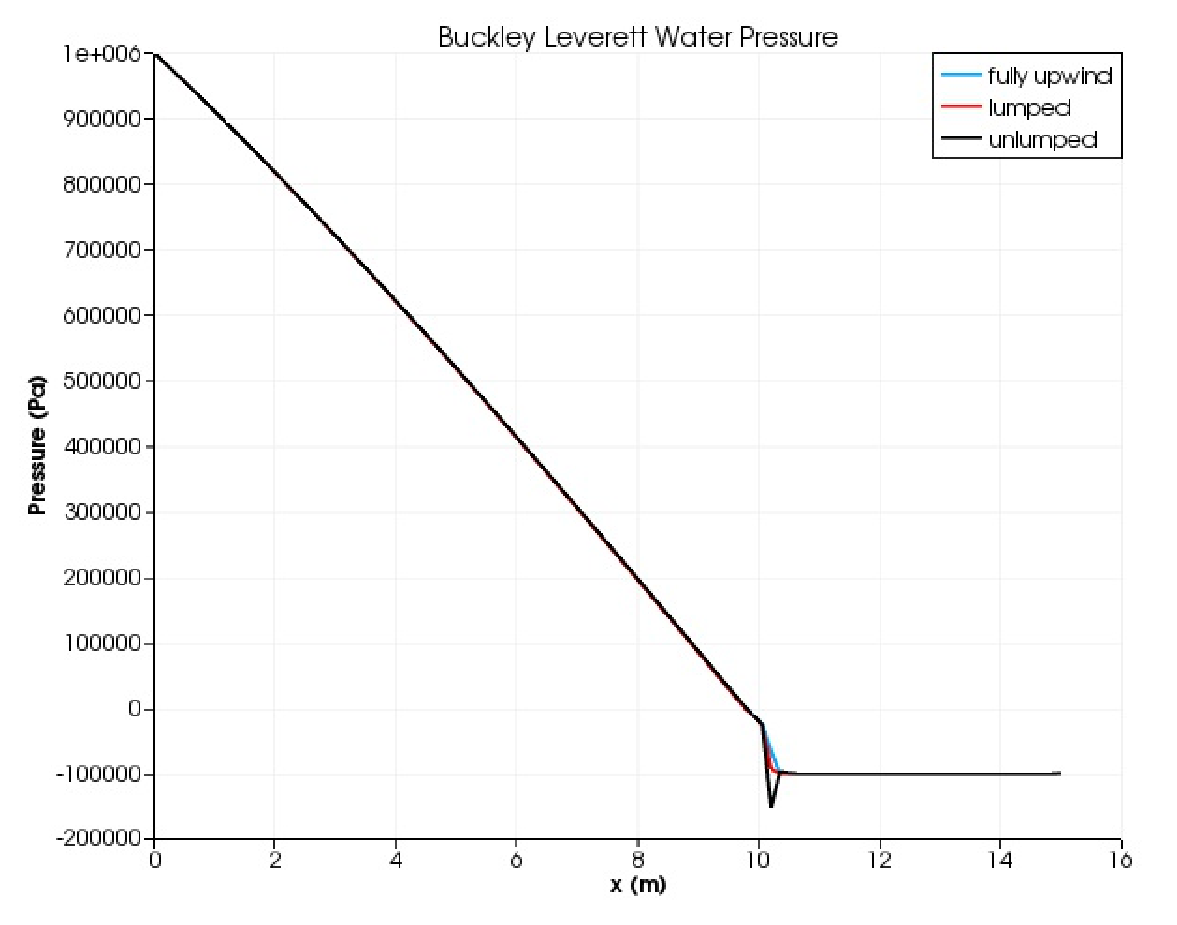
\includegraphics[width=7cm]{bl_lumped_unlumped.eps} &
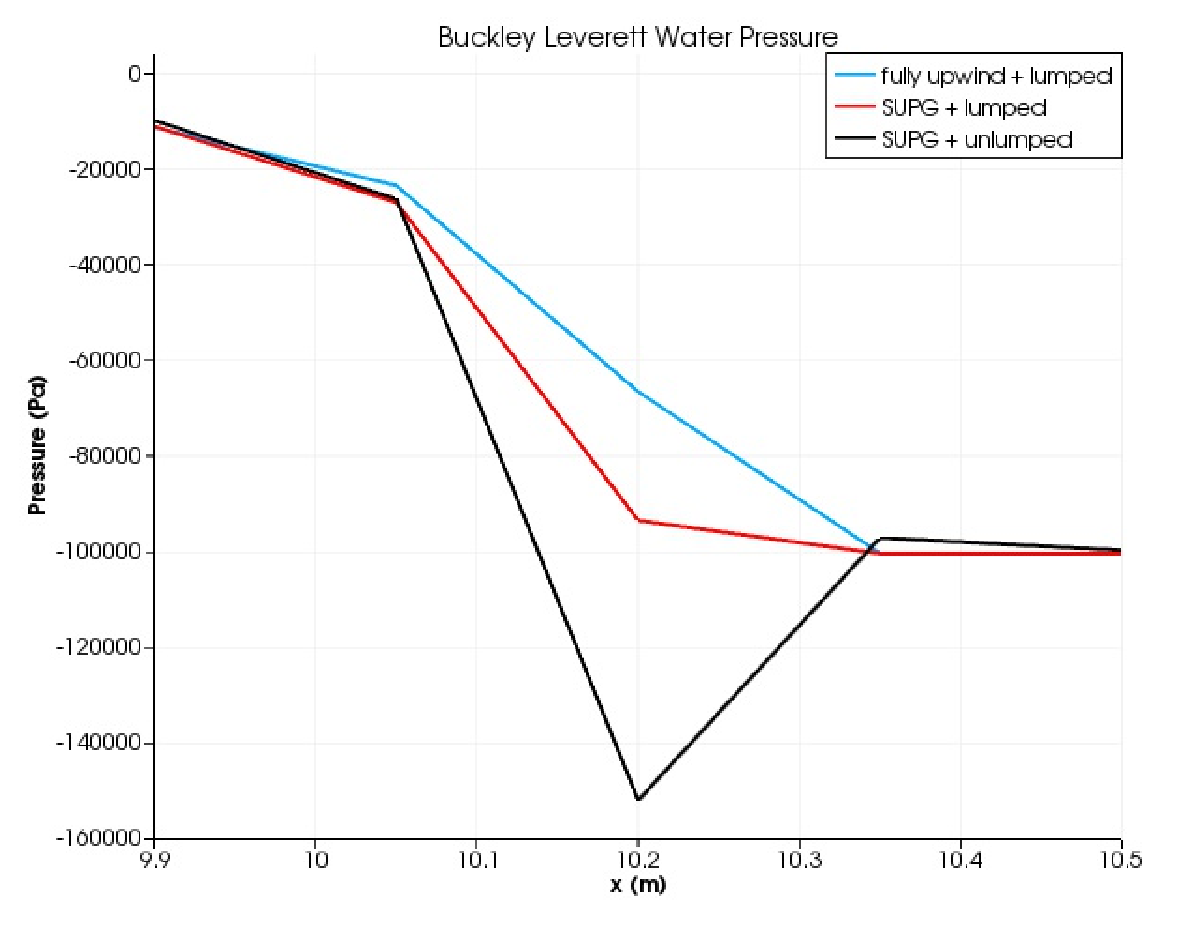
\includegraphics[width=7cm]{bl_lumped_unlumped_zoom.eps}
\end{tabular}
\caption{The water porepressure at $t=50$\,s in the Buckley Leverett
  problem.  Right: zoomed in on the region $x\rightarrow 10$.  Notice
  the oscillatory behaviour in the unlumped version.}
\label{bl_lump.fig}
\end{figure}




\chapter{Multi-phase Richards' equations}
\label{chap.multi}

The MOOSE implentation of Richards' equation is not only valid for the
single-phase case as described elsewhere in this document, but for the
multi-phase case too.  Denote the phase number by $\gamma$.  The
Richards' equations for multi-phase flow are
\begin{equation}
\phi \frac{\partial}{\partial t} \left( \rho^{\gamma} S^{\gamma} \right) = \nabla_{i}
\left( \frac{\rho^{\gamma} \kappa_{ij}\kappa^{\gamma}_{\mathrm{rel}}}{\mu^{\gamma}} (\nabla_{j}P^{\gamma} - \rho^{\gamma}
g_{j}) \right) 
+ F^{\gamma} \ ,
\label{richards.eqn.multi}
\end{equation}
where the independent variables are porepressures of the phases, $P^{\gamma}$.
The notation is the same as in Eqn~(\ref{richards.eqn}).

The MOOSE
implementation allows users to specify arbitrary functions for the
phase densities and relative permeabilities, but assumes the following.
\begin{itemize}
\item The density for phase $\gamma$ is only a function of its
  pressure: $\rho^{\gamma} = \rho^{\gamma}(P^{\gamma})$.
\item The relative permeability for phase $\gamma$ is only a function
  of its effective saturation: $\kappa^{\gamma}_{\mathrm{rel}} =
  \kappa^{\gamma}_{\mathrm{rel}}(S^{\gamma}_{\mathrm{eff}})$.
\end{itemize}
The immobile and relative saturations may be set independently for
each phase.

The effective saturations are more complicated, as they are functions
of all the pressure variables:
\begin{equation}
S^{\gamma}_{\mathrm{eff}} =
S^{\gamma}_{\mathrm{eff}}(P_{1},\ P_{2},\ldots) \ .
\end{equation}
It is therefore the saturations that couple the separate phases
together.  The MOOSE implementation allows users to specify arbitrary
functions for the effective saturations, but these must obey the
constraint 
\begin{equation}
\sum_{\gamma}S^{\gamma} = 1 \ .
\end{equation}

For two phases --- water and gas --- a common practise is to define
\begin{equation}
P_{c} = P_{\mathrm{gas}} - P_{\mathrm{water}} \ ,
\end{equation}
and to use the van Genuchten expression for the
water effective saturation:
\begin{equation}
S^{\mathrm{water}}_{\mathrm{eff}} = \left( 1 + (\alpha P_{c})^{\frac{1}{1 - m}}
\right)^{-m} \ \ \ \mbox{for}\ \ 0<m<1 \ .
\end{equation}
Then the gas effective saturation is just
$S^{\mathrm{gas}}_{\mathrm{eff}} = 1 -
S^{\mathrm{water}}_{\mathrm{eff}}$ (assuming residual saturations are
zero).  This common case has been coded and tested in the MOOSE implementation.





\chapter{Tolerances and Convergence}
\label{tol.chap}

It is sometimes difficult to set appropriate tolerances on the
nonlinear solver when running real models.  You should never expect
the nonlinear residual to go to exactly zero, because there will
always be problems associated with precision loss.  The absolute
tolerance on PETSc's nonlinear solver ({\tt{-snes\_atol}}) should be
set at the maximum of the numbers calculated below, otherwise
tolerance will never be achieved (unless it is through testing of the
relative sizes of the residuals).

\section{Minimum residual from spatial-derivative terms}
\label{sec.min.res.spat}

Consider the part of the residual
\begin{equation}
R = \int \psi \nabla_{i}
\left( \frac{\rho \kappa_{ij}\kappa_{\mathrm{rel}}}{\mu} (\nabla_{j}P
- \rho_{0} g_{j}) \right) \ .
\end{equation}
When discretised over the mesh this looks like
\begin{equation}
R_{\mathrm{element}} \sim L^{d} \frac{1}{L} \frac{\rho|\kappa|}{\mu}\frac{P_{1}-P_{0}}{L}
\ ,
\end{equation}
where $L$ is the element size, $d$ is the number of dimensions, and
$P_{1}$ and $P_{0}$ are the values of $P$ at neighbouring quadrature
points.  The relative permeability has been dropped because
$\kappa_{\mathrm{rel}}\leq 1$ and I want to place an upper bound on
the residual.

The key point is $P_{1}-P_{0}$ is subject to precision loss.  If, for
example $P_{1}=1$\,MPa, then $|P_{1}-P_{0}|\geq 10^{-15+6} =
10^{-9}$\,Pa, assuming that there are 15 digits of precision, and
barring the possibility that the computer has luckily converged upon
$P_{1}=P_{0}$ exactly.  This means that
\begin{equation}
R_{\mathrm{element}} \sim> 10^{-P}L^{d-2}\frac{\rho|\kappa|}{\mu}|P|
\ ,
\label{res.spatial.only}
\end{equation}
where $P$ is the number of digits of precision in the computer code.

{\underline{Example}} Suppose the user's model is expected to produce
pressures of a maximum of 10\,MPa, the density of their fluid is
approximately 1000\,kg.m$^{-3}$, the permeability tensor has
components of order $10^{-12}$\,m$^{2}$, the fluid viscosity is
$10^{-3}$\,Pa.s, and their elements are of size $L=100$\,m.  Then for
a 3D model with $P=15$ (double precision) the residual can never be
expected to fall below
\begin{equation}
R \sim 10^{-15}10^{2}\frac{10^{3}10^{-12}}{10^{-3}}10^{7} = 10^{-12}
\ .
\end{equation}
Clearly it is best to over-estimate the parameters in order to give a
maximum value for $R$, otherwise a model may apparently never
converge.  However, some judicious reasoning might be necessary if the
parameters in Eqn~(\ref{res.spatial.only}) vary substantially
throughout the mesh.


\section{Minimum residual from spatial-derivative terms with SUPG}

Consider the part of the residual
\begin{equation}
R = \int \tilde{\psi} \nabla_{i}
\left( \frac{\rho \kappa_{ij}\kappa_{\mathrm{rel}}}{\mu} (\nabla_{j}P
- \rho_{0} g_{j}) \right) \ .
\end{equation}
The standard part of this has been considered in
Section~\ref{sec.min.res.spat}.  The SUPG part of $\tilde{\psi}$ is
$\tau v_{i}\nabla\psi$, and $\tau |v|\sim L$, which gives
\begin{eqnarray}
R_{\mathrm{element}} & \sim & L^{d} L \left(\frac{\psi_{1}-\psi_{0}}{L}\right)
\left( \frac{\rho|\kappa|(0) - \rho|\kappa|(1)}{\mu L}\right)
\left(\frac{P_{1}-P_{0}}{L}\right)
\nonumber \\
& \sim & 10^{-2P} L^{d-2} \frac{\rho|\kappa|}{\mu}|P|
\ .
\end{eqnarray}
Evidently this is smaller than Eqn~(\ref{res.spatial.only}), so that
SUPG does not need to considered for the spatial-derivative terms.


\section{Minimum residual from temporal derivative terms}
\label{min.res.sec.temp}

Consider the part of the residual
\begin{equation}
R = \int \psi \phi \frac{\partial}{\partial t} \left( \rho S \right)
\ .
\end{equation}
When discretised over the mesh this looks like
\begin{equation}
R_{\mathrm{element}} \sim L^{d} \frac{\rho S_{\mathrm{d}t} - \rho
  S_{0}}{\mathrm{d}t} \ .
\end{equation}
The key point is that the time derivative of $\rho S$ is
subject to precision loss.  For instance, if $\rho S =
10^{3}$\,kg.m$^{-3}$, then $(\rho S_{\mathrm{d}t} - \rho S_{0}) \geq
10^{-15+3} = 10^{-12}$\,kg.m$^{-3}$.  This means that
\begin{equation}
R_{\mathrm{element}} \sim> 10^{-P}L^{d}{|\rho S|}/{\mathrm{d}t} \ .
\end{equation}
Notice that this depends on d$t$.  Hence when nonlinear-solving models
with very small timesteps, the residual may not reduce substantially
from its initial value!

{\underline{Example}}  Suppose the user's model has $S\sim 1$,
$\rho\sim 1000$\,kg.m$^{-3}$, elements of size $L\sim 100$\,m.  Then
for a 3D model with $P=15$ (double precision), the residual can never be expected to
fall below
\begin{equation}
R \sim 10^{-15}10^{6}\frac{10^{3}}{\mathrm{d}t} = 10^{-7}/{\mathrm{d}t}
  \ .
\end{equation}




\section{Minimum residual from temporal derivative terms with SUPG}

Consider the part of the residual
\begin{equation}
R = \int \tilde{\psi} \phi \frac{\partial}{\partial t} \left( \rho S \right)
\ .
\end{equation}
The standard part of this has been considered in
Section~\ref{min.res.sec.temp}.  The SUPG part of $\tilde{\psi}$ is
$\tau v_{i}\nabla_{i}\psi$ which is approximately $1$.  Hence the
addition of SUPG does not affect any considerations of minimum residual.






\addcontentsline{toc}{chapter}{\numberline{}Bibliography}
\bibliographystyle{unsrt}
\begin{thebibliography}{99}
\bibitem{richards1931}LA Richards ``Capillary conduction of
  liquids through porous mediums''   Physics 1 (1931) pp 318--333
\bibitem{vangenucthen1980}MT van Genuchten ``A closed-form equation
  for predicting the hydraulic conductivity of unsaturated soils''
  Soil Sci Soc Am J 44 (1980) 892--898.
\bibitem{bw1988}P Broadbridge and I White ``Constant rate rainfall
  infiltration: A versatile nonlinear model, 1 Analytical solution''.
  Water Resources Research 24 (1988) 145--154
\bibitem{rsc1983}C Rogers, MP Stallybrass and DL Clements ``On two
  phase filtration under gravity and with boundary infiltration:
  application of a Backlund transformation'' Nonlinear Analysis,
  Theory, Methods and Applications, 7 (1983) 785--799
\bibitem{peaceman1983}DW Peaceman ``Interpretation of well-block
  pressures in numerical reservoir simulation with nonsquare grid
  blocks and anisotropic permeability'' Society of Petroleum Engineers
  of AIME, June 1983, pp 531--543
\bibitem{chen2009}Z Chen and Y Zhang ``Well flow models for various
  numerical methods'' International Journal of Numerical Analysis and
  Modelling 6 (2009) 375--388
\bibitem{huyakorn1978}PS Huyakorn and GF Pinder ``A new finite element
  technique for the solution of two-phase flow through porous media''
  Advances in Water Resources 1 (1978) 285--298
\bibitem{dalen1979}V Dalen ``Simplified finite-element models for
  reservoir flow problems'' SPEJ (Oct 1979) 333--343
\bibitem{helmig1998}R Helmig and R Huber ``Comparison of Galerkin-type
  discretization techniques for two-phase flow in heterogeneous porous
  media''  Advances in Water Resources 21 (1998) 697--711
\bibitem{brooks1982}AN Brooks and TJR Hughes ``Streamline
  upwind/Petrov-Galerkin formulations for convection dominated flows
  with particular emphasis on the incompressible Navier-Stokes
  equations''  Computer Methods in Aplied Mechanics and Engineering 32
  (1982) 199--259.
\bibitem{hughesET1986}TJR Hughes, M Mallet and A Mizukami ``A new finite element
  formulation for computational fluid dynamics: II. Beyond SUPG''
  Computer Methods in Applied Mechanics and Engineering 54 (1986) 341--355
\bibitem{hughes1986}TJR Hughes and M Mallet ``A new finite element
  formulation for computational fluid dynamics: III. The generalized
  streamline operator for multidimensional advective-diffusive
  systems''  Computer Methods in Applied Mechanics and Engineering 58
  (1986) 305--328.
\bibitem{celiaET1990}MA Celia, ET Bouloutas and RL Zabra ``A general
  mass-conservative numerical solution for the unsaturated flow
  equation''  Water Resources Research 26 (1990) 1483--1496.
\end{thebibliography}





\end{document}

